% !TEX encoding = UTF-8 Unicode 
%
% Use:
% magister / inzynier - for master thesis or engineering thesis
% druk / archiwum - for print version or archive version
% en - to translate template into english
% examples:
%\documentclass[inzynier,druk,en] - master thesis, print version, english
%\documentclass[magister,druk,en]{dyplom}
%\documentclass[magister,druk]{dyplom}

\documentclass[inzynier,druk]{dyplom}

\usepackage[utf8]{inputenc}
\usepackage{hyperref}

% Maximum section's depth.
\setcounter{secnumdepth}{4}

% Listings settings
\setminted{breaklines, 
frame=lines,           
framesep=3mm,          
baselinestretch=1.1,   
fontsize=\small,       
% linenos              % line numbering
}

\usepackage{lipsum}

% \faculty{Faculty of \dots}                   % Uncomment if applicable
\fieldofstudy{Informatyka Techniczna (IMT)}                          
\author{Michał Gibas}
\title{System akwizycji i wstępnego przetwarzania sygnału EKG}
\supervisor{dr inż. Jacek Cichosz}
% \consultant{Consultant's name}               % Uncomment if applicable
% \specialisation{AAA}                         % Uncomment if applicable
\keywords{ekg, biosygnały, dsp}	% 3-5 keywords  

\begin{document}

\maketitle

\abstract{
Praca inżynierska koncentruje się na projekcie i realizacji urządzenia do akwizycji i przetwarzania elektrokardiogramu (EKG), 
wraz z opracowaniem oprogramowania urządzenia oraz aplikacji na komputery osobiste. 
Głównym celem jest stworzenie zintegrowanego systemu efektywnej 
rejestracji, analizy i wizualizacji sygnału EKG w czasie rzeczywistym. Urządzenie zawiera moduł wzmacniacza sygnału, mikrokontroler
do akwizycji i wstępnego przetwarzania oraz interfejs komunikacyjny z aplikacją. 
Oprogramowanie pozwala na wyświetlanie sygnału w czasie rzeczywistym oraz jego zapis.
}{
This thesis focuses on the design and implementation of a device used for electrocardiogram (EKG) aquisition and processing, 
along with the development of firmware for the device and an application for personal computers. 
The main goal is to create an integrated system for 
efficient recording, analysis, and real-time visualization of the EKG signal. The device includes a signal amplifier module, 
a microcontroller for acquisition and preprocessing, and a communication interface with the application. 
The software allows for the real-time display of the signal and saving it.
}



\tableofcontents

% !TEX encoding = UTF-8 Unicode 
% !TEX root = praca.tex

\chapter*{Wprowadzenie}

We współczesnym środowisku medycznym akwizycja i przetwarzanie biosygnałów,
w szczególności elektrokardiogramu (\textit{EKG}), stanowią kluczowe aspekty diagnostyki oraz
monitorowania zdrowia \cite{Serhani2020}. W świetle globalnej tendencji wzrostu 
przypadków zachorowań na przewlekłe choroby układu krążenia \cite{Gaidai2023}, 
rośnie zapotrzebowanie na tanie, efektywne i dostępne narzędzia diagnostyczne. 
Dostępność tych narzędzi, zwłaszcza w przypadku osób prywatnych oraz w warunkach słabo rozwiniętych 
systemów ochrony zdrowia, staje się poważnym wyzwaniem dla współczesnej medycyny \cite{Faruk2021}.

Przyjrzenie się obecnej sytuacji w obszarze medycyny ukazuje ograniczenia w dostępie do 
sprzętu oraz oprogramowania diagnostycznego, co jest szczególnie zauważalne w krajach rozwijających się \cite{Faruk2021}. 
W konsekwencji, potrzeba stworzenia prostych, tanich i powszechnie dostępnych narzędzi diagnostycznych, umożliwiających 
akwizycję i wstępne przetwarzanie sygnału \textit{EKG}, stała się motywacją oraz impulsem do podjęcia tematu tej pracy.

Przedstawione wyżej wyzwania podkreślają potrzebę rozwoju rozwiązań, które nie tylko zapewnią powszechny dostęp
do diagnostyki, ale również umożliwią błyskawiczną i efektywną analizę biosygnałów, wspierając tym samym szybkie 
i wczesne podejmowanie decyzji klinicznych. W ramach niniejszej pracy inżynierskiej, skoncentrowanej stworzeniu urządzenia 
oraz dedykowanego mu oprogramowania, zaproponowano prototyp taniego i dostępnego narzędzia diagnostycznego. 

Elektrokardiogram (\textit{EKG}) jest wynikiem aktywności elektrycznej serca, spowodowanej skurczem i rozkurczem tego mięśnia 
\cite{Limaye2016}. Sygnał \textit{EKG} jest funkcją mierzonego napięcia w czasie. 
Jeden cykl składający się ze skurczu i rozkurczy, reprezentowany jest przez zespoł tzw. \textit{załamków} 
oznaczonych literami \textit{P}, \textit{Q}, \textit{R}, \textit{S} i \textit{T} przedstawionymi na rys \ref{fig:pqrst}.

Zasadniczą trudnością w systemach akwizycji i przetwarzania sygnałów jest efektywna eliminacja zakłóceń (\textit{szumów}), które
znacząco utrudniają proces diagnostyczny w przypadku sygnału \textit{EKG}. Wśród nich wyróżnić można m. in. \cite{Limaye2016}: 
dryft linii izoelektrycznej (\textit{baseline wander}), 
szumy indukowane przez instalacje elektryczne w budynkach (\textit{power line interference noise}) 
czy artefakty spowodowane ruchem pacjenta. Jedną ze sprawdzonych metod eliminacji szumów są filtry cyfrowe, w tym filtry 
o skończonej odpowiedzi impulsowej \textit{FIR} (\textit{Finite Impulse Response}) \cite{Tompkins1993}.

\begin{figure}[h!]
    \centering
    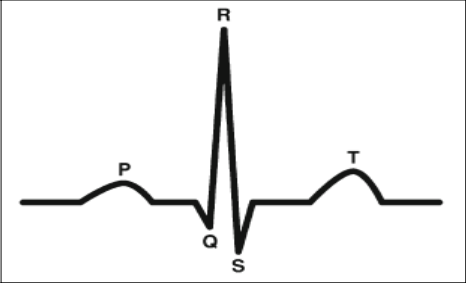
\includegraphics[scale=0.6]{pl/media/pqrst.png}
    \caption{Zespoł załamków \textit{PQRST} (\cite{Limaye2016}, fig. 1.)}
    \label{fig:pqrst}
\end{figure}

\newpage

\section*{Cel i zakres pracy}

Celem pracy było stworzenie sprzętowego oraz programowego systemu akwizycji i wstępnego przetwarzania sygnału \textit{EKG} 
mającego znamiona narzędzia diagnostycznego. W zamyśle pracy było stworzenie prototypowego systemu przeznaczonego 
do użytku prywatnego, w tym do wstępnej i samodzielnej oceny stanu mięśnia sercowego a następnie
potencjalnej konsultacji lekarskiej.  
Autor zastrzega jednak, że praca ma wymiar edukacyjny, a celem jej nie było stworzenie narzędzia diagnostycznego spełniającego 
standardy urządzenia medycznego.


Niniejsza praca opisuje projekt i realizację dwóch części:

\begin{itemize}

    \item \textbf{sprzętowej}: makieta układu elektronicznego\footnote{Przez makietę rozumiany jest prototyp urządzenia typu 
    \textit{PoC} (ang. \textit{Proof of Concept})}, zawierająca układ wzmacniacza, filtry analogowe, 
    mikrokontroler, programator sprzętowy oraz mostek \textit{USB}/\textit{UART},


    \item \textbf{programowej}: oprogramowanie sprzętowe (inaczej \textit{firmware}), aplikacja na komputery PC 
    (zwana w dalszych rozdziałach \textit{aplikacją}) oraz programy/skrypty wspomagające projektowanie filtrów cyfrowych 
    (zwane krócej \textit{skryptami}).

\end{itemize}

Część sprzętowa odpowiada za wstępne wzmocnienie i analogową filtrację sygnału \textit{EKG} 
oraz umożliwienie komunikacji z komputerem PC na którym zainstalowana jest wspomniana aplikacja. 


Oprogramowanie sprzętowe (na układ mikrokontrolera makiety sprzętowej) umożliwiło obsługę przetwornika analogowo/cyfrowego,
implementację filtrów cyfrowych oraz implementację protokołu oraz obsługę interfejsu do komunikacji z komputerem PC.
Aplikacja na komputery PC została stworzona w celu podglądu sygnału oraz jego zapisu w czasie rzeczywistym.

\newpage

\section*{Użyty sprzęt oraz technologie}

Ze względu prototypowy charakter pracy, część sprzętowa zrealizowana została jako makieta w oparciu o gotowe
płytki drukowane z układami elektronicznymi. W skład części sprzętowej wchodzą następujące elementy, szczegółowiej
opisane w rozdziale 2:

\begin{itemize}

    \item płytka z układem \textbf{AD8232} \cite{AD8232BS} \cite{AD8232ds}: zawiera filtry analogowe oraz układ wzmacniaczy,


    \item płytka z mikrokontrolerem \textbf{STM32F411} oraz programatorem \textbf{STLink v2} \cite{STM32F4DS} \cite{NUCLEO}: 
    zawiera mikrokontroler z mikroprocesorem \textit{ARM Cortex M4} oraz układami peryferyjnymi takimi jak: 
    przetwornik analogowo/cyfrowy, liczniki czy kontroler \textit{DMA} (\textit{Direct Memory Access}),
    

    \item przewody połączeniowe, w tym przewód \textit{USB} do połączenia makiety z komputerem PC.


\end{itemize}

W części programowej użyto następujących języków, bibliotek i narzędzi:

\begin{itemize}

    \item \textbf{język C} (standard \textit{C11}): język kompilowany użyty w implementacji oprogramowania sprzętowego,

    \item \textbf{język C++} (standard \textit{C++20}): język kompilowany użyty w implementacji 
    protokołu komunikacyjnego oraz aplikacji,

    \item \textbf{ARM GNU Embedded Toolchain} \footnote{\url{https://developer.arm.com/downloads/-/gnu-rm}}: zestaw narzędzi, w tym
    kompilatorów języków \textit{C} i \textit{C++} oraz \textit{assemblera} dla mikroprocesorów \textit{ARM Cortex-M},

    \item \textbf{biblioteka STM32HAL} \cite{STM32HAL}: biblioteka dostarczająca warstwę abstrakcji dla mikroprocesora 
    oraz układów peryferyjnych mikrokontrolera \textit{STM32F411}.

    \item \textbf{SDL2} \cite{SDL2}: biblioteka umożliwiająca renderowanie rastrowej grafiki dwuwymiarowej zastosowana
    do implementacji wykresu sygnału w aplikacji,

    \item \textbf{standardowe biblioteki języków C i C++ na system GNU/Linux} \cite{GLIBC238}: biblioteki użyte do 
    implementacji komunikacji międzyprocesowej, wielowątkowości oraz niektórych struktur danych w aplikacji,

    \item \textbf{język Python 3} \footnote{\url{https://www.python.org/}}: język skryptowy użyty do napisania 
    skryptów obliczeniowych i pomocniczych w projektowaniu filtrów cyfrowych,
   
    \item \textbf{CMake} \footnote{\url{https://cmake.org/}} \textbf{oraz GNU Make} 
    \footnote{\url{https://www.gnu.org/software/make/}}: systemy automatyzujące 
    kompilację i linkowanie aplikacji w \textit{C} i \textit{C++}.

\end{itemize}



% !TEX encoding = UTF-8 Unicode 
% !TEX root = praca.tex

\chapter{Opis systemu}

Rozdział ten poglądowo opisuje system będący przedmiotem pracy, z naciskiem na 
wysokopoziomowy opis systemów. 
Poszczególne elementy systemu zostały przedstawione na schemacie poglądowym na rys. \ref{fig:hl_sys}.

\begin{figure}[h!]
    \centering
    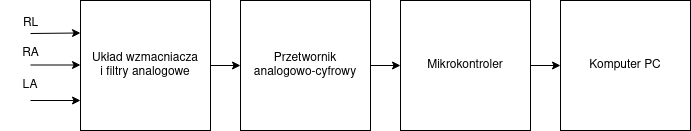
\includegraphics[scale=0.6]{pl/media/hl_system.png}
    \caption{Schemat poglądowy systemu}
    \label{fig:hl_sys}
\end{figure}

Do pomiaru aktywności elektrycznej serca zastosowano klasyczny układ 3 elektrod pomiarowych używany często
w diagnostyce arytmii \cite{FRANCIS201692}, z oznaczeniami \textit{RL} (\textit{right leg}, prawa noga), 
\textit{RA} (\textit{right arm}, prawa ręka) oraz \textit{LA} (\textit{left arm}, lewa ręka). W tej 
konfiguracji elektrody można umieścić w sposób jaki sugerują oznaczenia tzn. na kończynach lub alternatywnie 
na klatce piersiowej (\textit{RA} i \textit{LA}) oraz poniżej żeber (\textit{RL}). 
Istnieje możliwość zmiany umiejscowienia elektrod tak aby utworzyć inne konfiguracje, które również umożliwiają akwizycję sygnału
mającego wartość w diagnostyce chorób serca.

\begin{figure}[h!]
    \centering 
    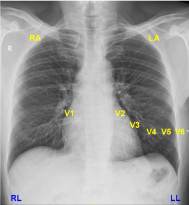
\includegraphics[scale=1.2]{pl/media/electrodes.png}
    \caption{Zdjęcie rentgenowskie klatki piersiowej wraz z oznaczeniami\\ dla 3-elektrodowej konfiguracji oraz oznaczeniami dodatkowymi
    \cite{FRANCIS201692}(\textit{Fig. 1.})}
    \label{fig:ele}
\end{figure}

\newpage

\section{Wzmocnienie sygnału i filtracja analogowa}

Sygnał \textit{EKG} charakteryzuje się małymi amplitudami, w zakresie od dziesiątek do setek $\mu V$ \cite{Zywietz1990}.
Ta cecha badanego sygnału uniemożliwia dokonywanie bezpośredniego pomiaru w sposób dokładny przez klasyczne przetworniki analogowo/cyfrowe (\textit{ADC}, \textit{Analog to Digital Converter})
ze względu na ich niską rozdzielczość. Jako rozwiązanie w pracy zastosowano zestaw wzmacniaczy w układzie scalonym firmy \textit{Analog Devices}, \textit{AD8232} \cite{AD8232ds}. 
Ze względu na to że mierzone impulsy mogą mieć wartości ujemne, \textit{AD8232} przesuwa, wzmacnia i normalizuje amplitudę sygnału w taki sposób że sygnał wyjściowy znajduje się w przedziale od $0V$ do $3,3V$co umożliwia próbkowanie i jego kwantyzację za pomocą klasycznych przetworników \textit{ADC}. 
\textit{AD8232} zapewnia również mechanizm wykrywania podłączonych elektrod (ang. \textit{leads off detection}).


W pracy użyto płytki drukowanej z układem \textit{AD8232} \cite{AD8232BS} w konfiguracji z dwoma pasywnymi filtrami analogowymi: 
górnoprzepustowym oraz dolnoprzepustowym, o wynikowym paśmie przepuszczania $[0,5 Hz; 40Hz]$ (rys. \ref{fig:afilt}) \cite{AD8232ds}.
Filtry analogowe złożone w części z elementów biernych (rezystorów, kondensatorów i cewek) nie są idealne ze względu na wahania w 
parametrach tych elementów związane m.in. z temperaturą czy starzeniem się elementów. Kolejnym problemem staje się kwestia połączeń
między przetwornikiem ADC a mikrokontrolerem. Każda ścieżka lub przewód sygnałowy są podatne na szumy pochodzące z otoczenia, będące
wynikiem np. indukcji elektromagnetycznej \cite{EmcPhy2010}. Jednym z rozwiązań wymienionych problemów mogą być 
filtry cyfrowe, które nie są tak podatne na fizyczne warunki pracy jak ich analogowe odpowiedniki.

\begin{figure}[h!]
    \centering 
    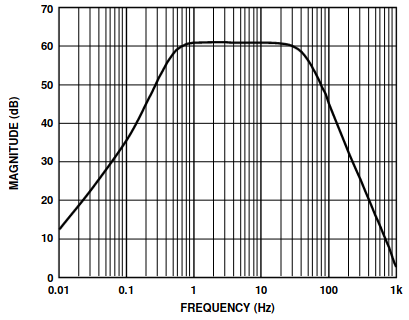
\includegraphics[scale=0.75]{pl/media/afilt.png}
    \caption{Wykres charakterystyki częstotliwościowej zastosowanego układu filtrów analogowych podany przez producenta \cite{AD8232ds}(\textit{Fig. 67.})}
    \label{fig:afilt}
\end{figure}

\newpage

\section{Próbkowanie, kwantyzacja i komunikacja z komputerem osobistym}

Do próbkowania i kwantyzacji sygnału zastosowano wbudowany w układ scalony mikorkontrolera \textit{STM32F411CE} przetwornik analogowo/cyfrowy o rozdzielczości 12 bitów \cite{STM32F4DS}.
Na podstawie literatury \cite{Ajdaraga2018} ustalono, że częstotliwość próbkowania $f_{s}$ o wartości $360 Hz$ dla sygnału \textit{EKG} spełnia zarówno założenia twierdzenia o próbkowaniu
jak i wymagania diagnostyczne.


W pracy użyto wbudowanego w \textit{STM32F411CE} kontrolera \textit{DMA} (\textit{Direct Memory Access}), umożliwiającego
transfery danych między przetwornikiem \textit{ADC} a pamięcią \textit{SRAM} w sposób niezależny od rdzenia mikrokontrolera. 
Umożliwiło to równoległe przetwarzanie danych trafiających do bufora w pamięci przez rdzeń \textit{ARM Cortex M4}. 
Próbkowanie z częstotliwością $f_{s}$ zrealizowano za pomocą wbudowanego
układu licznika cyfrowego w konfiguracji generującej przerwanie co okres $T_{s} = \frac{1}{f_s}$, każde przerwanie rozpoczyna kolejną konwersję przetwornika
\textit{ADC} oraz następujący po nim transfer próbki poprzez \textit{DMA}.
\textit{STM32F411CE} posiada rdzeń procesora \textit{ARM Cortex M4} który w swojej architekturze 
(\textit{ISA}, \textit{Instruction Set Architecture}) zawiera również instrukcje użyteczne w cyfrowym przetwarzaniu sygnałów (\textit{DSP}, \textit{Digital Signal Processing}) \cite{CM4DSP} takie jak np.: 
operacje na liczbach zmiennoprzecinkowych czy
instrukcje typu \textit{SIMD} (\textit{Single Instruction Multiple Data}).


Komunikację z komputerem osobistym zrealizowano za pomocą interfejsu \textit{UART} (\textit{Universal Asynchonous Receiver/Transmitter}). 
Wbudowany w programator \textit{ST Link} układ mostka \textit{UART/USB}, umożliwił komunikację z użyciem \textit{UART} poprzez fizyczny interfejs \textit{USB} w komputerze osobisty.
W celu zapisu i podglądu sygnału zaprojektowano i zaimplementowano aplikację okienkową na system operacyjny \textit{GNU/Linux} 
dla architektury standardowych komputerów osobistych (\textit{x86\_64}).
Aplikację zaprojektowano z myślą o komunikacji ze sprzętem poprzez standardowe sterowniki 
np. \textit{cdc\_acm} \footnote{\url{https://github.com/torvalds/linux/blob/master/drivers/usb/class/cdc-acm.c}}
dla systemu \textit{Linux} w wersji \textit{6.5}.



% !TEX encoding = UTF-8 Unicode 
% !TEX root = praca.tex

\chapter{Makieta sprzętowa}

\cite{AD8232ds}


% !TEX encoding = UTF-8 Unicode 
% !TEX root = praca.tex

\chapter{Oprogramowanie sprzętowe}

\section{Wstęp i wymagania funkcjonalne}
Oprogramowanie makiety sprzętowej stworzono z myślą o następujących wymaganiach funkcjonalnych:

- zapewnienie komunikacji z komputerem PC poprzez interfejs \textit{UART},

- wykrycie podłączenia elektrod i adekwatna zmiana koloru diody \textit{RGB},

- odczyt próbkowanych i kwantyzowanych wartości z przetwornika \textit{ADC},

- wstępne przetwarzanie sygnału przy użyciu filtrów cyfrowych.  

Oprogramowanie sprzętowe napisano głównie w języku \textit{C}, w nieznacznej cześci przy 
pomocy języka \textit{C++}. W implementacji zastosowano również bibliotekę \textit{HAL STM32},
która służyła jako warstwa abstrakcji między sprzętem a oprogramowaniem. Do preprocessingu, 
kompilacji i konsolidacji użyto narzędzi z kolekcji \textit{ARM GNU Embedded Toolchain}. 
Użyto również programów do automatyzacji procesu
budowania oprogramowania takich jak \textit{CMake} oraz \textit{GNU Make}.

\textit{Firmware} był wgrywany do pamięci \textit{EEPROM} 
(\textit{Electrically Erasable Programmable Read-Only Memory}) mikrokontrolera za pomocą
programatora sprzętowego \textit{STLink}.
Programator podłączano poprzez interfejs \textit{USB} do komputera \textit{PC}.
Do przesyłania obrazu pamięci w postaci
pliku binarnego użyto oprogramowania dostarczonego przez producenta: \textit{st-flash} 
\cite{stflash}. Na listingu \ref{listing:stflash} przedsatwiono przykładowe wywołanie wspomnianego
programu, gdzie \textit{ECGMonitor.bin} to binarny obraz programu, natomiast \textit{0x8000000} to
adres (liczba szesnastkowa z prefiksem \textit{0x}) 
pod który zostanie załadowany obraz.

\begin{listing}
\begin{minted}{bash}
st-flash write ECGMonitor.bin 0x8000000
\end{minted}
\caption{Wywołanie programu st-flash do  programu na mikrokontroler}
\label{listing:stflash}
\end{listing}

Po zakończeniu wszystkich kroków procesu budowania \textit{firmwareu} wynikowym plikiem
jest plik ELF (\textit{Executable Linkable Format}) \cite{elfARM}. 
Plik ten zawiera m.in. informacje na temat segmentów programu czy dodatkowych symboli 
do \textit{debugowania}. Format ten jednak nie jest kompatybliny z narzędziem \textit{st-flash}.
Narzędzie to przyjmuje binarny obraz pamięci, który załadowywany jest począwszy od wskazanego
w linii poleceń adresu. Do wygenerowania obrazu pamięci z pliku \textit{ELF}, zastosowano program 
\textit{arm-none-eabi-objcopy} z kolekcji \textit{ARM GNU Embedded Toolchain}.

\section{Akwizycja sygnału}

W oprogramowaniu sprzętowym użyto wbudowanego w mikrokontroler kontrolera \textit{DMA}, który połączony jest
osobną od rdzenia magistralą z innymi układami peryferyjnymi i pamięcią. Umożliwia to niemal niezależne
transfery danych między przetwornikiem analogowo-cyfrowym a pamięcią.
W celu osiągnięcia precyzyjnej częstotliwości próbkowania $f_s = 360 Hz$ wykorzystano wbudowany układ licznika
o rozdzielczości 16 bitów, który skonfigurowano by zliczał w naturalnym kodzie binarnym modulo 512 z częstotliwością 
$f_c \approx 184,3 kHz$ i generował przerwanie przy każdym przepełnieniu. W kontrolerze przerwań skonfigurowano ten 
typ przerwania w taki sposób aby każdorazowo wywoływało konwersję przetwornika analogowo-cyfrowego, a przewanie
końca konwersji wywoływało transfer \textit{DMA} z przetwornika do bufora kołowego w pamięci mikrokontrolera.
W rutynie przerwania sygnalizującego koniec transferu \textit{DMA} umieszczono fragment kodu przedstawiony na listingu
\ref{listing:dmairq}.

\begin{listing}
\begin{minted}{c}
__disable_irq();
adc_buffer_last_index = (adc_buffer_last_index + 1) % ADC_BUF_LEN;
__enable_irq();
\end{minted} 
\caption{Fragment rutyny przerwania dla zakończenia transferu \textit{DMA} z przetwornika \textit{ADC} do pamięci}
\label{listing:dmairq}
\end{listing}

Funkcje \textit{\_\_disable\_irq} i \textit{\_\_enable\_irq} odpowiadają kolejno za tymczasowe wyłączanie obsługi przerwań 
i jej ponowne włączenie.
Zmienna \textit{adc\_buffer\_last\_index} przechowuje indeks na którym zostanie zapisana kolejna próbka w buforze kołowym, będącym
tablicą o długości \textit{ADC\_BUF\_LEN} i rozmiarze elemtów równym dwóm bajtom (rozmiar każdej z próbek). Wartość
indeksu jest inkrementowana, dzięki operacji modulo nie przekracza zakresu tablicy i wraca na jej początek po dotarciu do końca.
Wspomniane \textit{\_\_disable\_irq} i \textit{\_\_enable\_irq} funkcje zastosowanu w tym przypadku aby zapewnić 
atomowość operacji inkrementacji indeksu w buforze kołowym, innymi słowy by nie dopuścić innych przerwań do 
potencjalnego opóźnienia tak krytycznej dla działania sprzętu operacji.


Odczyt danych z bufora kołowego odbywa się przy założeniu że rdzeń odczytuje próbki z bufora kołowego na tyle szybko,
że nigdy nie dojdzie do sytuacji gdy dane jeszcze nieodczytane zostaną nadpisane nowymi. Do śledzenia indeksu odczytu
zdefiniowano zmienną globalną \textit{adc\_buffer\_curr\_index}, na rysunku \ref{fig:rbuffer} przedstawiono bufor
kołowy w skrajnym przypadku gdzie jest on zapełniony i w przypadku nieodczytania danych dostatecznie szybko, dane zostaną utracone.
Podobnie jak w przypadku \textit{adc\_buffer\_last\_index}, wspomniana zmienna globalna jest inkrementowana przy każdym odczycie
wraz z wykonaniem analogicznej operacji modulo.

\begin{figure}[h!]
    \centering 
    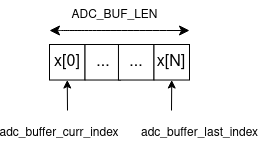
\includegraphics[scale=0.7]{pl/media/rbuffer.png}
    \caption{Rysunek poglądowy bufora kołowego zwierającego próbki sygnału}
    \label{fig:rbuffer}
\end{figure}

\newpage
\section{Implementacja filtrów FIR}

Obecność jednostki zmiennoprzecinkowej \textit{FPU} (\textit{Floating-point Unit}) w rdzeniu \textit{ARM Cortex M4} 
mikrokontrolera umożliwia szybkie operacje na liczbach zmiennoprzecinkowych bez konieczności implementacji tych operacji 
w oprogramowaniu. Z racji na to zdecydowano, że współczynniki filtrów \textit{FIR} przechowywane będą w pamięci 
mikrokontrolera jako liczby zmiennoprzecinkowe pojedynczej precyzji w standardzie \textit{IEEE-754}. Użycie typu
zmiennoprzecinkowego umożliwia łatwe przeniesienie współczynników wyliczonych podczas projektowania filtru na mikrokontroler.

\begin{listing}
\begin{minted}{c}
#include <inttypes.h>

typedef float fp32_t;

struct fir_t
{
  const fp32_t* coeffs;
  uint32_t coeffs_len;
  volatile uint16_t* buf;
  uint32_t buf_len; 
};
\end{minted} 
\caption{Struktura fir\_t}
\label{listing:firt}
\end{listing}

Na listingu \ref{listing:firt} przedstawiono strukturę przekazywaną potem do funkcji realizującej dyskretny splot sygnału z
współczynnikami filtru. Pole \textit{coeffs} jest wskaźnikiem (adresem) na stałą tablicę współczynników zapisaną w pamięci
mikrokontrolera ustawianą podczas kompilacji oprogramowania, zawartą w wynikowym w pliku wykonywalnym wgrywanym do pamięci 
\textit{EEPROM} mikrokontrolera. Pole \textit{buf} jest wskaźnikiem do bufora kołowego zawierającego próbkowany sygnał.
Natomiast pola \textit{coeffs\_len} oraz \textit{buf\_len} oznaczają odpowiednio długości tablic: 
współczynników oraz bufora kołowego.
Pole \textit{buf} wymaga dopisanego słowa kluczowego \textit{volatile} ze względu na naturę zapisów do wspomnianego bufora: poprzez
przerwania i transfery DMA. 


W wypadku buforów modyfikowanych przez rutyny przerwań lub inne mechanizmy sprzętowe 
pojawia się następujący problem: kompilator języka \textit{C} nie posiadając kontekstu i informacji na temat architektury maszyny
na jakiej program będzie wykonywany, traktuje rutyny przerwań jako funkcje które nigdy nie zostają wywołane. Zatem jeżeli do zapisu
danych do bufora nie dochodzi w innych częściach programu, to kompilator może zoptymalizować wszystkie odczyty danych 
z bufora poprzez wstawienie we wspomniane miejsca instrukcji odczytania zera przechowanego np. w rejestrze procesora, 
zamiast kosztownego odczytu z pamięci. Słowo kluczowe \textit{volatile} jest sugestią dla kompilatora, aby ten nie przeprowadzał
optymalizacji w przypadku danego fragmentu pamięci, adresu, zmiennej lub funkcji.


Działanie filtru FIR implementuje funkcja \textit{fir\_convolve} przedstawiona na listingu \ref{listing:firconv}. 
Funkcja ta realizuje operację splotu dyskretnego próbek sygnału ze współczynnikami flitru:

$$
(f * g)[n] = \sum_{k=-\infty}^{\infty} f[k]g[n-k]
$$

\begin{listing}
\begin{minted}{c}
fp32_t fir_convolve(struct fir_t* fir, uint32_t pos)
{ 
    uint32_t buf_idx = pos; 
    fp32_t result = 0.0f;
  
    for(uint32_t c_idx = fir->coeffs_len; c_idx != 0 ; --c_idx) { 
        result += (fir->buf[buf_idx] * fir->coeffs[c_idx - 1]);
        buf_idx = (buf_idx + 1) % fir->buf_len;
    }     
  
    return result;
} 
\end{minted} 
\caption{Funkcja realizaująca splot dyskretny próbek sygnału ze współczynnikami filtru FIR}
\label{listing:firconv}
\end{listing}

\newpage

\section{Wykrywanie podłączonych elektrod}

Układ \textit{AD8232} udostępnia dwa wyprowadzenia do wykrywania odłączonych elektrod oznaczone \textit{LOD-} i \textit{LOD+}.
W wypadku gdy jedna lub więcej elektrod jest niepodłączona to conajmniej jedno z wyprowadzeń jest w stanie wysokim 
(logiczna 1).
Wykrywanie podłączonych elektrod zrealizowano dzięki możliwości generowania przerwań zewnętrznych poprzez wykrycie zmiany
stanu wyprowadzenia mikrokontrolera. Wyprowadzenia (połączone z \textit{LOD-} i \textit{LOD+}) w odpowiednich portach 
wejścia/wyjścia ogólnego przeznaczenia (\textit{GPIO}, \textit{General Purpose Input/Output})
skonfigurowano tak, aby generowały przerwanie przy wykryciu zbocza opadającego lub narastającego. 
Dla obu tych przerwań zewnętrznych w wektorze przerwań ustawiono ten sam adres rutyny obsługującej przerwanie.

\begin{listing}
\begin{minted}{c}
void EXTI9_5_IRQHandler(void)
{
  if( (HAL_GPIO_ReadPin(LOD_N_GPIO_Port, LOD_N_Pin) == 0) &&
      (HAL_GPIO_ReadPin(LOD_P_GPIO_Port, LOD_P_Pin) == 0) )
  {
    __disable_irq();
    HAL_GPIO_WritePin(LED_RED_GPIO_Port, LED_RED_Pin, 1);
    HAL_GPIO_WritePin(LED_GREEN_GPIO_Port, LED_GREEN_Pin, 0);
    leads_off = false;
    __enable_irq();
  }
  else
  {
    __disable_irq();
    HAL_GPIO_WritePin(LED_RED_GPIO_Port, LED_RED_Pin, 0);
    HAL_GPIO_WritePin(LED_GREEN_GPIO_Port, LED_GREEN_Pin, 1);
    leads_off = true;
    __enable_irq();
  }
\end{minted} 
\caption{Fragment rutyny obsługi przerwania zewnętrznego 
          realizujący wykrywanie odłączonych elektrod}
\label{listing:leadsoff}
\end{listing}

Fragment kodu wspomnianej procedury osbługi przerwania przedstawiono na listingu \ref{listing:leadsoff}.
Funkcje z przedrostkiem \textit{HAL\_GPIO\_} są funkcjami biblioteki \textit{HAL STM32}. Funkcja
\textit{ReadPin} odczytuje wartość logiczną danego wejścia w danym porcie \textit{GPIO}, natomiast
\textit{WritePin} ustawia zadaną wartość na wyjściu danego wyprowadzenia. W programie użyto zmiennej globalnej
\textit{leads\_off}, która gdy jest równa prawdzie, oznacza że elektrody nie są podpięte prawidłowo do ciała pacjenta.
W przypadku wykrycia odłączenia kolor diody \textit{RGB} na płytce z mikrokontrolerem ustawiany jest na czerwony, w
przeciwnym wypadku na kolor zielony (konkretne kolory aktywowane są wartością \textit{0}).

\section{Komunikacja z użyciem interfejsu UART}

Dla prostoty komunikacji urządzenia z komputerem PC zastosowano komunikację jednokierunkową,
urządzenie wysyła dane poprzez interfejs zawsze kiedy wykryje podpięte elektrody a w buforze kołowym znajdują 
się nowe próbki do odczytu.



% !TEX encoding = UTF-8 Unicode 
% !TEX root = praca.tex

\chapter{Aplikacja na komputery PC}



% !TEX encoding = UTF-8 Unicode 
% !TEX root = praca.tex

\chapter{Projekt i implementacja filtrów cyfrowych}


% !TEX encoding = UTF-8 Unicode 
% !TEX root = praca.tex

\chapter*{Podsumowanie}

\section{Osiągnięte rezultaty}

Podsumowując, w niniejszej pracy udało się zrealizować postawione cele.
Zaprojektowano i stworzono funkcjonalny prototyp urządzenia oraz oprogramowanie sprzętowe.
Stworzono również aplikację na komputery osobiste, która ułatwia korzystanie z urządzenia.
Główne osiągnięcia pracy obejmują:

1. Opracowanie i wykonanie modułu akwizycji sygnału: zaprojektowanie i wykonanie
makiety sprzętowej składającej się ze wzmacniacza analogowego oraz mikrokontrolera,
co umożliwiło efektywną akwizycję sygnału EKG.

2. Rozwój oprogramowania:
zaprojektowano i zaimplementowano filtry cyfrowe, minimalizując tym samym wpływ zakłóceń 
na jakość sygnału. Stworzona aplikacja umożliwiła podgląd sygnału w czasie rzeczywistym
oraz jego zapis do pliku.

3. Testowanie i walidacja systemu:
przeprowadzono testy manualne potwierdzające że urządzenie działa stabilnie i zgodnie
z oczekiwaniami.

\section{Perspektywy rozwoju}

Rozwój projektu urządzenia jak i oprogramowania otwiera możliwości usprawnienia i dodania 
nowych funkcji. Poniżej przedstawiono niektóre z możliwych dróg rozwoju pracy w przyszłości:

1. Dodanie akumulatora (np. litowo-jonowego) oraz modułu \textit{WiFi} umożliwiając 
bezprzewodowe działanie sprzętu: wprowadzenie zasilania bateryjnego wraz z komunikacją
radiową mogłoby przekształcić urządzenie w przenośny, bezprzewodowy system monitorowania
serca pacjenta, w podobny sposób jak robią to współczesne urządzenia nazywane \textit{holterami}.

2. Udoskonalenie interfejsu użytkownika aplikacji: interfejs tekstowy na którym opierają się 
główne części aplikacji (pomijając okienko wykresu w czasie rzeczywistym) 
nie jest intuicyjnym i prostym interfejsem dla przeciętnego użytkownika.
Rozwój bardziej przejrzystego, graficznego środowiska, z użyciem tzw. \textit{widgetów}
może okazać się o wiele łatwiejszy w obsłudze.

\newpage

3. Projekt płytki PCB i obudowy urządzenia: opracowanie dedykowane płytki drukowanej (\textit{PCB})
i ergonomicznej obudowy pozwoli na miniaturyzację urządzenia, zwiększając jego praktyczność
i trwałość. Projekt dedykowanej płytki drukowanej pozwoli również na zmniejszenie podatności 
na zakłócenia zewnętrzne. 

4. Opracowanie oprogramowania i sprzętu zgodnego ze standardami urządzeń medycznych:
współcześnie, urządzenia medyczne muszą spełniać szeregi standardów bezpieczeństwa i jakości.
Każde takie urządzenie jest akceptowane (lub nie) przez odpowiednie komisje, które dopuszczają
produkt do użycia w środowisku medycznym.

5. Klasyfikacja chorób przy pomocy modeli uczenia maszynowego: metody uczenia maszynowego
mogą okazać się przydatne w procesie diagnostycznym i wspomagać badania przesiewowe.
Wśród nich przykładowo sieci neuronowe mogą posłużyć do klasyfikacji występowania 
arytmii w rejestrowanym sygnale w czasie rzeczywistym.


\nocite{*}

% Bibliography
\bibliographystyle{dyplom}
\bibliography{thesis_refs}


% Lists of figures, listings, tables
\listoffigures
\listoflistings
\listoftables

\end{document}
